% ===============================================================
%
% For tracking purposes - this is V2.0 - May 2012

\documentclass{sig-alternate}
\usepackage{float}
\floatstyle{boxed}
\newfloat{pseudocode}{h}{lop} %{chapter}
\floatname{pseudocode}{\textbf{Algorithm}}
\usepackage{amsfonts}
\usepackage{amsmath}
%\usepackage{amsthm}
\usepackage{amstext}
\usepackage{amssymb}
\usepackage{algorithmic}
\usepackage{fainekos-macros}  
\usepackage{amsbsy}
\usepackage{graphicx}
\usepackage{todonotes}
\usepackage{enumerate}      
\usepackage{fixltx2e}
%\usepackage{ifthen} 
%\usepackage{bigdelim,multirow,xspace}
%\newtheorem*{IEEEproof}{Proof}
%********************************************************************
\graphicspath{{figures/}}

\newcommand{\agentInstanceSet}{A}
\newcommand{\agentTypeSet}{\Ac}
\newcommand{\scenarioSet}{S}
\newcommand{\exitConditions}{\Ec}
\newcommand{\lawSet}{\Lc}

\begin{document}
%
% --- Author Metadata here ---
\conferenceinfo{EMSOFT}{2015 Amsterdam, The Netherlands}
%\CopyrightYear{2007} % Allows default copyright year (20XX) to be over-ridden - IF NEED BE.
%\crdata{0-12345-67-8/90/01}  % Allows default copyright data (0-89791-88-6/97/05) to be over-ridden - IF NEED BE.
% --- End of Author Metadata ---

\title{When you have more than a hammer: multi-formalism verification of autonomous plans}

\maketitle

%\begin{abstract}
%Autonomous and semi-autonomous systems are now an accepted part of the economy and society, whether they are autonomous robots in shipping warehouses or autonomous appliance robots in the home.
%The success of these robots can be attributed, in part, to the fact that either they function in highly controlled environments where their interactions with other agents are structured, or their tasks are simple enough to accommodate unstructured and unpredictable environments.
%In this paper, we develop a framework for formally verifying the safety of autonomous systems operating in unstructured environments in the presence of other unpredictable agents. 
%Using autonomous vehicles as a running example, 
%we present a decomposition of an autonomous system's mission into scenarios and agents, and a rich representation of these two elements in terms of hierarchical communicating hybrid automata. 
%Our goal is to formally verify that the behavior of the autonomous system is safe in a given scenario, which possibly involves other unpredictable (nondeterministic) agents.
%Therefore, we include in our framework a translator from this rich representation into the formalisms of various formal verification tools, to enable the use of the most appropriate tool for a given verification task. 
%The fact that multiple tools are needed is illustrated with the verification of the safety of a lane change maneuver, which requires the use of a timed automaton verification tool, and a rechability tool.
%Another goal is to allow control engineers to use these formal tools as part of their design process. 
%Therefore, we develop a scenario authoring tool, and a domain-specific language with formal semantics, for enabling rapid prototyping and verification of controllers' designs.
%


\end{abstract}

% A category with the (minimum) three required fields
\category{H.4}{Information Systems Applications}{Miscellaneous}
%A category including the fourth, optional field follows...
\category{D.2.8}{Software Engineering}{Metrics}[complexity measures, performance measures]

\terms{Theory}

\keywords{ACM proceedings, \LaTeX, text tagging}

% Start here
\section{outline}
\label{outline}
\todo[inline]{this section will be removed from final paper, of course}
Introduction
\begin{itemize}
	\item The benefits of autonomous systems.
	
	\item The acceptance of autonomous systems in the economy and our daily lives.
	
	\item Autonomous vehicles as a running example. What are the "real-world" challenges? (e.g. lane change in some detail, then just list others like pedestrians, other drivers,etc)
	
	\item What are the technical challenges facing the development of autonomous vehicles? (e.g. properties with priorities)
	
	\item How are these challenges addressed in today's technology and literature?
	
	\item What remains to be done?
	
	\item Which piece of the puzzle are we addressing in this paper? Illustrate with the running example of a lane change maneuver.
	
	\item How are we addressing it?
	
	\item The need for formal methods.
\end{itemize}



Modeling framework
\begin{itemize}
	\item Scenarios and agents (don't dwell too long on this, just need to mention that we are verifying one scenario in this paper, but we have a plan for how this fits with overall mission verification)
	
	\item HCHA: because we need a representation rich enough to express on it different types of properties, which apply to different components of the complex autonomous vehicle
	
	\item Specification languages: should be suited to the verification goal. Here, reachability and LTL

\end{itemize}

Lane change in the formalisms.
\begin{itemize}	
	\item Formal model of lane change in terms of HCHA for system, LTL for scenario goal, and reach sets for safety. Controller is a discrete controller in grid world.
	
	\item Lane change requirements can be verified with timed automata, so need to translate HCHA. Give translation.
	
	\item How results are mapped back to HCHA
	
\end{itemize}


Experiment
\begin{itemize}
	\item Experimental setup: simulation or actual little vehicles? UPPAAL, dReach, make it available online
	
	\item results
	
\end{itemize}

Future work
\begin{itemize}
	\item Tool chain: from design entry to formal DSL (implementing HCHA) to design files for relevant tools
	\item priority of requirements?
\end{itemize}
\section{Introduction}
\label{introduction}

{\it Autonomy from human intervention in the machines that surround us promises many benefits.}

{\it Because of these benefits, autonomous and semi-autonomous systems are now an accepted part of the economy and the household.}

{\it Autonomous vehicles are a particularly challenging class of autonomous systems.}

{\it On a typical trip, the autonomous vehicle must recognize, enter, complete and exit many scenarios in a safe and timely manner. Example scenarios include traffic lights, roundabouts, pedestrians, weather conditions, etc. 
It is not known, ahead of time, what the specific sequence of encountered scenarios will be.}

{\it The corresponding technical challenges can be broadly divided into two categories: operation in a highly unpredictable environment, and a task (navigation) that must be executed at many levels of abstraction.}

{\it The environment of the autonomous vehicle is unpredictable: will others obey the laws, what will traffic conditions be, etc? What is the vehicle's objective in the short run?}

{\it There is also a wide separation between the highest levels of plan execution ("go from A to B") and the lowest levels of plan execution ("accelerate steadily for the next 5 seconds"). How do we guarantee consistency between the commands at the different levels?}

{\it The safety of the car's passengers and of the people in its immediate environment is imperative at all times. 
	What does safety mean in a given scenario?
	In an emergency, how do we recognize what laws can be broken to preserve safety?}

\todo[inline]{Safety,comfort,performance}
%\footnote{Interesting legal question: if the car, by design, violates some law to avoid harming someone, how long before the manufacturer gets sued for purposefully breaking the law? Think about swerving too hard and "losing control of the vehicle" to avoid running over someone.}
%\footnote{Other notions of safety, such as passive safety where the autonomous system must not endanger others via \emph{inaction}, or extensions of the safety imperative to not damaging property (and not just people) are not covered here. We note nonetheless that guaranteeing that the active safety imperative is obeyed contributes to guaranteeing these other notions are also obeyed.}
%For people to feel comfortable interacting with potentially dangerous autonomous agents, like autonomous cars, it is imperative that they be confident that these systems are at least as safe as the human-operated systems they are replacing.
%In fact, for there to be an economic value behind the introduction of autonomous systems, they must, among other things, guarantee an increased level of safety relative to the current system. 
%Increased and more consistent efficiency and effectiveness at completing their tasks are other desiderata, which are outside the scope of this paper.
%We call this the `dorasical' environment, from the Greek $\delta \rho \acute{\alpha} \sigma \eta$ for action.


{\it Guaranteeing safety to a socially acceptable degree requires formal guarantees.}

{\it Today we have theories that deal with high-level planning in a discrete grid world: where the car should go given where everyone else is.}

{\it We also have discrete theories for verification of temporal logic properties of the closed-loop system modeled as a Kripke structure. Some of these theories are amenable to model checking.}

{\it Control theory provides analysis and design tools of low level controllers. Automatic analysis tools exist but are limited in scope.}

{\it Because of the large degree of unpredictability, compute- and memory-intensive low level methods can't be used alone (let alone manual methods). Yet because of the safety imperative, we can't rely on non-guaranteed abstractions.  In this paper, we demonstrate the need for using multiple formalisms in the verification of autonomous plans. We illustrate this with a case study of a typical lane change maneuver.}

\begin{exmp}[Lane change maneuver]
	
	Throughout this work we will take as a case study the following example. At various instances we will zoom in on on specific scenarios within the sequence of events. The case study shows a target vehicle driving on a two lane road network that includes a merge which introduces another vehicle into the path of the target vehicle. The target vehicle's planning system may autonomously decide to initiate a lane change manuever to get around the other vehicle. The scenario terminates with an intersection governed by a traffic light. This scenario contains two vehicle agents (with different plans, 1 traffic control (infrastructure agent), and 1 road network. 
	
	\todo[inline]{who's involved in this scenario; what is the goal of ego vehicle; what is the sfaety constraint; why model checking alone won't suffice.}
\end{exmp}

From a planning perspective we define the safety of the discrete controller of the target vehicle to be the satisfaction of the following safety and liveness properties:
\begin{enumerate}
	\item The target vehicle may not exceed the speed limit (safety).
	\item The target vehicle may not collide with any other vehicles (if they exist) on the road (safety).
	\item The target vehicle must stop at a red light (safety).
	\item The target vehicle must eventually complete the scenario (liveness).
It is clearly possible to specify these properties using LTL operators (always and eventually).
\end{enumerate}

%Work on autonomous navigation: DARPA urban challenge papers, controller synthesis papers.
%
%DSL: that paper by the french authors, others?
%
%Scenarios and agents: there has to be a tonne here...the papers referenced by Matt in the APEX preso
%
%Interaction between model checkers and other verif tools: CEGAR, matthias and CMU guy, spaceex.
%
%Other semi-formal verif: staliro, breach, apx bisimulations.

\subsection{Notation}
We denote the set of integers including 0 with $\Ne$. 
Given a subset $S$ of the reals, $S^* = S \setminus \{0\}$ and $S_+ = S \cap [0,\infty)$,
while $S_+^* = S \cap (0,\infty)$.
\section{Agent models}
\label{HCHA}

In this section we define the mathematical models of agents involved in a scenario: Hierarchical Communicating Hybrid Automata (HCHA).
Not all agents will require the full generality of HCHA, but having a general model allows us to specialize it in various ways to suit the agent and the scenario. 
In addition, it will be possible for us to abstract from the HCHA to system models that are amenable to the formal verification techniques at our disposal. 
As noted in the introduction, the execution of an autonomous plan involves many levels of abstraction. The verification must cover all these levels.

We start with a few basic elements:
an agent (of one of the types described above) has a state vector $\stPt \in \reals^n$.
(Different agents may have different dimensions.)
The state includes all information of relevance to the system designers.%: for the ego vehicle, this will typically include position and velocity, but also fuel combustion rate and wall-wetting effects if needed.
%For a traffic light (which is an agent of type \texttt{trafficSignage}), the state might include the current active light and a clock that measures the delay between light switches.
An agent is modeled as a \emph{communicating} hybrid automaton.

\begin{defn}[Communicating hybrid automaton]
	\label{def:CHA}
A driven \textbf{communicating hybrid automaton} (CHA) $\Sys$ with inputs in $\inpSet$ 
is a tuple 
\[\Sys = (\stSet, \modeSet, E, Inv, \{F_\mode\}_{\mode \in \modeSet}, \guard, \reset, \funcOut, C)\]
where 
\begin{itemize}
	\item $\stSet \subseteq \Re^n$ is the continuous state space of the system.
	\item $\modeSet \subset \Ne$ is a finite set of control locations that the system switches through. 
	\item $\hsSet \triangleq \modeSet \times \stSet$ is then the hybrid state space.
	\item $F_\mode : \stSet \times \inpSet \rightarrow \Re^n$ defines a differential inclusion governing the evolution of the state in location $\mode$: $\dot{\stPt} \in F_\mode(\stPt,u)$. 
	\item $Inv : \modeSet \rightarrow 2^\stSet$ defines an invariant condition on the state while in location $\mode$: $\stPt \in Inv(\mode)$.
	\item $E \subseteq \modeSet \times \modeSet$ is the set of location transitions (a.k.a. switches, or jumps).
	%
	\item $\guard : E \rightarrow 2^\stSet$ is the guard condition that enables a location transition. 
	Namely, the system switches between $\mode _i$ and $\mode _j$ when the state $\stPt$ is in $\guard((\mode_i,\mode _j))$.
	%
	\item $\reset : E \times \stSet \rightarrow \modeSet \times \stSet $ is a reset map that, given a transition $e = (\mode _i,\mode _j) \in E$ and a point $x$ on the guard $\guard(e)$, maps $x$ to a point $x^+$ in the invariant set of the next location $\mode_j$:
	\[\reset: ((\mode _i,\mode _j),x) \rightarrow (\mode_j,x^+)\;, x^+ \in Inv(\mode_j)\] 
	%
	\item $\funcOut: \reals^n \rightarrow \reals^p$ is an output function,
	\item $C = \{c_1,\ldots,c_{p_C}\}$ is a set of $p_C \in \Ne$ perception conditions (defined below).	
\end{itemize}
\end{defn}

The differential inclusion $F_\mode$ in each location of the CHA models the continuous-time closed-loop behavior of the physical controlled systems.%, e.g., the electromechanical systems of the car such as the powertrain.
The state $\stPt$ captures all the relevant information about the agent's dynamics. 
It is widely recognized now that different navigation situations call for different control laws.
\todo[inline]{cite}
This is modeled by the locations of the CHA: each location represents the application of a different control law that is appropriate for the situation.

The solutions of regular ODEs are given as functions of the independent variable time $t$.
Because hybrid automata also include a discrete evolution of the state (namely, via the reset map $\reset$), their solutions will be given as a function of time $t$ and jump number $j$.
We first define hybrid time domains and arcs.
\begin{defn}[Hybrid time domains and arcs~\cite{GoebelT06_SolnsHybInclusions}]
	\label{def:hybridarcs}
	A subset $E \subset \Re_+\times \Ne$ is a \emph{compact hybrid time domain} if 
	\[E = \bigcup_{j=0}^{J-1}[t_j,t_{j+1}]\times \{j\}\]
	for some finite increasing sequence of times $0=t_0 \leq t_1 \leq t_2 \leq \ldots \leq t_J$.
	We say $E$ is a \emph{hybrid time domain} if for all $(T,J) \in E$, 
	$E \cap ([0,T]\times \{0,\ldots,J\})$ is a compact hybrid time domain.
	Define
	$\sup_t E = \sup \{t \sut \exists (t,j) \in E\}$, $\sup_j E = \sup \{j \sut \exists (t,j) \in E\}$,
	and $E.last = (\sup_t E, \sup_j E)$.
	
	A \emph{hybrid arc} $\hstraj$ is a function supported over a hybrid time domain $\hstraj:E \rightarrow \Re^n$, 
	such that for every $j$, $t \mapsto \hstraj(t,j)$ is absolutely continuous in $t$ over $I_j = \{t: (t,j) \in E\}$;
	we call $E$ the domain of $\hstraj$ and write it $\dom \hstraj$.
	%The \emph{graph} of a hybrid arc is the set $\gph \hstraj = \{(t,j,\hstraj(t,j)): (t,j) \in \dom \hstraj\}$.
	Finally, $\dom_t \hstraj = \proj{\dom \hstraj}{\nnreals}$ and $\dom_j \hstraj = \proj{\dom \hstraj}{\Ne}$
\end{defn}

Note that each $I_j$ is an interval.
%$E.last$ indicates the last element of $E$ under the linear order $(t,j) \leq (t',j')$ iff $t \leq t'$ and $j\leq j'$.
As observed in \cite{SanfeliceT10automatica}, hybrid time domains are equivalent to hybrid time trajectories used in \cite{LygerosJSZS03tac} to define executions of hybrid automata.
Output and state trajectories of hybrid automata will be modeled as hybrid arcs. 

Given a hybrid automaton $\Sys$ and a point $\hsPt_0  = (\mode_0, \stPt_0)$, 
a \emph{solution} $\hstraj_{\hsPt_0}$ of $\Sys$ (aka \emph{state trajectory}) is given by a hybrid arc $\hstraj$ 
satisfying the following conditions:
\begin{enumerate}
	\item $\hstraj_{h_0}(0,0) = h_0$
	\item $\hstraj_{h_0}(t,j) = (\mode(t,j),\sttraj(t,j)) \in \hsSet \; \forall (t,j) \in \dom \hstraj$
	\label{item:explicitLX}
	\item For each $j$ s.t. $I_j$ has a non-empty interior, 
	\[\dot{\sttraj}(t,j) \in F_{\mode(t,j)}(\sttraj(t,j))\]
	for almost all $t \in I_j$, and $\sttraj(t,j) \in Inv(\mode(t,j))$ for all $t \in \text{int}I_j$.
	Moreover, 
	\begin{equation*}
	\label{eq:zeroderiv}
	\dot{\mode}(t,j) = 0 \; \forall t \notin \{ \inf I_j, \sup I_j\}
	\end{equation*}
	\label{item:contevolutions}
	\item For all $j$ s.t. $(t,j) \in \dom \hstraj$, $(t,j+1) \in \dom \hstraj$, it holds that $\sttraj(t,j) \in \guard(\mode_i,\mode_k)$ for some $i,k$,
	$\sttraj(t, j+1) = \reset(\sttraj(t,j), (\mode_i,\mode_k))$,
	and $\sttraj(t,j+1) \in Inv(\mode_j)$.
	\label{item:jumpHA}
\end{enumerate}
See Fig.~\ref{fig:HA} for an illustration.
We consider that the discrete time variable $j$ simply counts the location changes (via \eqref{eq:zeroderiv} and Condition \ref{item:jumpHA}).
The transition itself between locations takes 0 real time.
The location changes can only occur when the continuous state $\stPt$ enters a guard set (Condition \ref{item:jumpHA}). 
The sequence of control locations that the trajectory $\hstraj$ visits is denoted by $\loc(\hstraj)$.

If $\hstraj$ is a state trajectory, then $\funcOut \circ \hstraj: \dom \hstraj \rightarrow \hsSet$ is called an \emph{output trajectory}.
We assume that $\funcOut$ is such that an output trajectory is also a hybrid arc, supported on the same hybrid time domain as the corresponding state trajectory:
$\dom \hstraj = \dom \funcOut \circ \hstraj$.

\begin{figure}[tb]
	\centering
	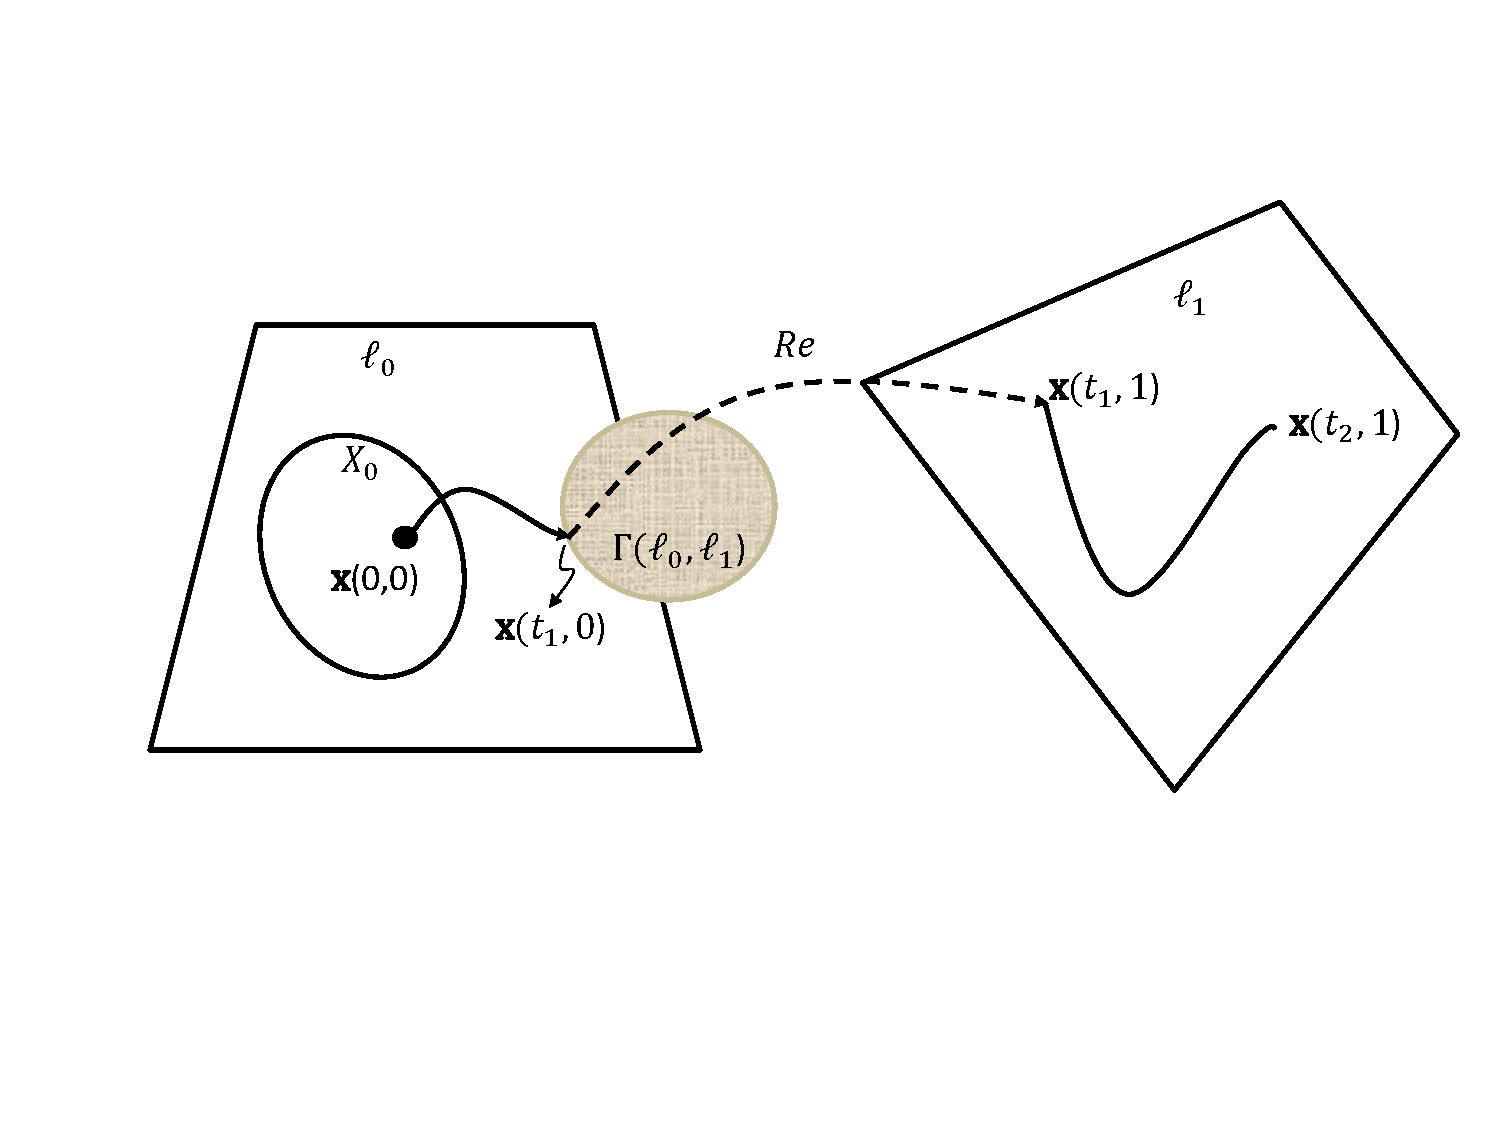
\includegraphics[scale=0.4]{figures/HA.pdf}
	\caption{State trajectory of a hybrid automaton.}
	\label{fig:HA}
\end{figure}

\begin{defn}
	\label{def:solutionsets}
	$\Sc_\Sys(\hsPt_0)$ will denote the set of solutions of $\Sys$ with initial condition $\hstraj(0,0) = \hsPt_0$,
	and $\Sc_\Sys$ will denote the set of all solutions of $\Sys$.
	A hybrid automaton is said to be \emph{deterministic} if $\Sc_\Sys(\hsPt_0)$ is a singleton for any $\hsPt_0$.
\end{defn}

We will use $\hstraj_\hsPt$ to refer to the trajectory starting at $h$.
The system has a finite set of initial locations $\modeSet_0 \subset \modeSet$ in which it could start, 
and within each such location $\mode$, a set of initial continuous states $\stSet_\mode \subset \stSet$ in which it could start. 
Any solution to the system's equations must start there. We denote 
\[H_0 = \bigcup_{\mode \in \modeSet_0} \{\mode\}\times \stSet_\mode\]
the hybrid initial set, and write
\[Init = \bigcup_{\mode \in \modeSet_0}\stSet_\mode \]


\begin{exmp}[Lane change continued]
	We model the lane change scenario using HCHA as follows
	\todo[inline]{must show how the 4 agent types are modeled with this}
	\end{exmp}


\subsubsection{Abstraction levels}
\label{abstractionLevelsOfHCHA}

We formally define the abstraction levels at which it is controlled, and consequently at which it is verified.
A \emph{hierarchical} CHA is a CHA with a chain of partitions defined on its location set $\modeSet$, and a corresponding chain of simplified continuous dynamics.
\begin{defn}[Hierarchical CHA]
	\label{def:HCHA}
	A \textbf{hierarchical CHA} (HCHA) is a tuple 
	$(\Sys, \{V_i\}_{i=0}^{a}, \{P_i\}_{i=0}^{a}, \{\Sys_i\}_{i=0}^{a})$ where 
	$\Sys$ is an $n$-dimensional CHA, 
	each $V_i$ in the chain 
	\[V_a \subset V_{a-1} \subset \ldots \subset V_1 \subset V_0=\{1,\ldots,n\}\]
	is the set of \emph{surviving variables} at level $i$, and 
	$\{P_0,P_1,\ldots,P_a\}$ is an ascending chain of partitions of the set $\modeSet$, that is:
	\begin{itemize}
		\item $P_0 = \modeSet$
		%
		\item For every $i =1,\ldots,a$, $P_i \subset 2^\modeSet$ partitions $\modeSet$: $[\mode] \cap [\mode'] = \emptyset$ for all $[\mode],[\mode'] \in P_i$ and $\cup_{\mode\in \modeSet}[\mode] = \modeSet$
		%
		\item For all $i<a$, for all $[\mode]\in P_i, \exists [\mode'] \in P_{i+1}$ s.t. $[\mode] \subset [\mode']$ 
	\end{itemize}
	Every element of $\{\Sys_i\}_{i=1}^{a}$ is an $n_i$-dimensional CHA 
	\[\Sys_i = (\stSet_i, \modeSet_i, E_i, Inv_i, \{F_{q,i}\}_{q \in \modeSet_i}, \guard_i, \reset_i, \funcOut_i, C_i)\]
	where  $\Sys_0 = \Sys$,
	$n_i \geq n_{i+1}$,
	\begin{eqnarray*}
		\modeSet_i &=& P_i
		\\
		(q,q') \in E_i &\text{ iff }& \exists \mode \in q, \mode' \in q' \text{ s.t. } (\mode,\mode') \in E_{i-1}		
		\\
		\stSet_i & = & \proj{\stSet_{i-1}}{V_i} 
		\\
		\guard_i((q,q')) &=& \proj{\cup_{(\mode,\mode') \in q\times q'} \guard_{i-1}((\mode,\mode')) }{V_i}
		\\
		Inv_i(q) &=& \proj{ \cup_{\mode \in q}Inv_{i-1}(\mode)}{V_i}
		\\
		F_{q,i}(x) &\supset & \proj{\cup_{\mode \in q}F_{\mode,i-1}(x^\uparrow)}{V_i}
		\\
		\reset_i(e,x) &=& \proj{\cup_{e' \subset e}\reset_{i-1}(e',x^{\uparrow})}{V_i}
		\\
		\forall x \in \stSet_{i-1},\; \proj{x}{V_i} &=& \proj{\reset_{i-1}(e,x)}{V_i}
		\\
		C_i &=& C
		\end{eqnarray*}
Finally, for all $ e \in E_{i-1},x \in \guard_{i-1}(e)$,
\[\proj{x}{V_i} = \proj{\reset_{i-1}(e,x)}{V_i}\]
		
\end{defn}
\todo[inline]{should $F$ be the convex hull of the union?}
Every element $P_i$ of the partition chain represents an abstraction level. 
An element $[\mode]$ of $P_i$ is a `super-mode' which aggregates several modes of $P_{i-1}$ (namely, the elements of $P_{i-1}$ in the equivalence class $[\mode]$).
The state vector is reduced in dimension by projecting the state vector at abstraction level $i-1$ onto the variables $V_i$ of the new level. 
The set $V_i$ is part of the data of the HCHA.
For example, it may consist of the state variables that appear in the guard conditions leading out of the super-modes $q \in \modeSet_i$.
The guards and invariants are defined accordingly, by doing the same projection for all guard and invariant conditions on a given transition in $\Sys_{i-1}$.
The new level's dynamics $F_i$ are part of the data of $\Sys_i$. 
For example, they may be obtained by Model Order Reduction from the dynamics of $\Sys_{i-1}$, or some domain-specific transformation.
The input set is correspondingly modified.
Note that by imposing $C_i=C$ we impose that the variables involved in each perception condition survive all levels.
This is a reasonable assumption when we consider that perception conditions involve physical quantities that can be perceived by other agents in the environment, and therefore are unlikely to be dropped by designers as `irrelevant' at some level of abstraction. 
\begin{rem}
	It is possible to define successive abstraction levels to perform more elaborate mappings on the state vector than simple projections, and the rest of the paper would follow with some simple modifications. 
		We define the HCHA with projections because this is more typical of the manner in which different design teams design their systems, with attention paid to the quantities of interest at their level, while assuming that lower levels somehow provide them with readings (or computations) of this data.
\end{rem}


\todo[inline]{add HCHA fig and mention of fig to clarify}

To formally state the relation between executions at different abstraction levels, we must first define executions of hybrid automata. 

\begin{thm}
	Let $(\Sys,\Vc,\Pc,\{\Sys_i\})$ be a HCHA.
	Let $\hstraj =(\mode,\sttraj) \in \Sc_{\Sys}$ be a solution of CHA $\Sys$ with continuous part $\sttraj$.
	Then for every $1 \leq i \leq a$, 
	there exists a solution 
	$\hstraj^{(i)} = (q,\sttraj^{(i)}) \in \Sc_{\Sys_i}$ 
	such that $\sttraj^{(i)} = \proj{\sttraj}{V_i}$.
	That is, for every $(t,j) \in \dom \hstraj$, there exists $(t,j') \in \dom \hstraj^{(i)}$
	s.t. $\mode(t,j) \in q(t,j')$
	and	$\sttraj^{(i)}(t,j) = \proj{\sttraj(t,j')}{V_i}$.
\end{thm}

\begin{proof}
	We prove this for $i=1$. The general case follows by induction.
	Fix $i=1$, and write $V$ for $V_i$ in this proof.
	Let $\sttraj$ be as stated, and define 
	$y: \dom \sttraj \rightarrow \reals^{n_i}$ by 
	$y(t,j) = \proj{\sttraj(t,j)}{V}$ for all $(t,j) \in \dom \sttraj$.
	We will construct from $y$ a hybrid arc that satisfies the conditions of a solution of $\Sys_i$.
	
	Let $I_j$ be an interval in $\dom \hstraj$ with non-empty interior, and take $t \in I_j$ s.t. 
	$\dot{\sttraj}(t,j) \in F_\mode(\sttraj(t,j))$. 
	Then $\dot{y}(t,j) = d(\proj{\sttraj(t,j)}{V})/dt = \proj{\dot{\sttraj}(t,j)}{V} \in \proj{F_\mode(\sttraj(t,j))}{V} \subset F_q(y^{\uparrow}(t,j))$.	
	For all $t \in \text{int}I_j$, $y(t,j) = \proj{\sttraj(t,j)}{V} \in \proj{Inv(\mode)}{V} = Inv(q)$.
	Moreover, for all $t$ different from the endpoints of $I_j$, $q(t,j) = [\mode]$ and so $\dot{q}(t,j) =0$.
	Thus condition 3 is satisfied for $y$.
	
	Now consider the jumps: let $t_r = \sup I_J$. 
	If the jump at $(t_r,j)$ leads from $\mode$ to a location $\mode'$ such that $[\mode']$ is not $q$, then it can be shown that this is also a jump for $y$.
	However, if the transition is \emph{internal} to mode $q$, i.e. 
	\[[\mode]=[\mode']\]
	then this violates condition 4 since $y(t_r,j)$ is not in a guard set of $\Sys_i$.
	Moreover, because of the reset that occurs at $(t_r,j)$, if $\proj{\sttraj(t_r,j+1)}{V}\neq \proj{\sttraj(t_r,j)}{V}$, then $y$ is not absolutely continuous as a function of time within each mode.
	To get around these difficulties, we invoke the last property defining an abstraction chain.
	Namely, that the surviving variables at each level are not affected by resets on internal transitions.
	This removes the second difficulty above since now $y(t_r,j+1) = y(t_r,j)$.
	
	We define $\sttraj^{(i)}$ by erasing the internal transitions from the domain of $y$.
	Let $\Jc$ be the set of indices of internal transitions, that is, $\Jc = \{j \sut \exists t.(t,j) \in \dom \sttraj, (t,j+1) \in \dom \sttraj, [\mode(t,j)]=[\mode(t,j+1)]\}$.		
	
	\todo[inline]{TBC}
\end{proof}

\todo[inline]{initial points}

\begin{thm}
	Let $(\Sys,\Vc,\Pc,\{\Sys_i\})$ be a HCHA.
	Let $y \in \Sc_{\Sys_i}$ be a solution of CHA $\Sys_i$ for some $i$.
	Then either there exists $\sttraj \in \Sc_\Sys$ s.t. $y} = \proj{\sttraj}{V_i}$,
	or $y$ can be refined to such a trajectory in at most $|\modeSet|\cdot n$ steps,
	where $\modeSet$ is the location set of $\Sys$ and $n$ is its dimension.
\end{thm}

\begin{proof}
	Write $y$ for Assume that a solution $\sttraj$ as stated does not exist.
	There are two reasons why this might happen:
	\begin{itemize}
		\item Either, iwithin the same $I_j$ in the domain of $y$, $\dot{y}$ obeys two different dynamics $F_\mode$ and $F_{\mode'}$ for $\mode,\mode' \in q \in \modeSet_i$.
		In general, this can not be produced by a $\Sys$ trajectory.\footnote{}
	\end{itemize}
\end{proof}
%
%\subsubsection{Inputs and perception conditions}
\label{inputsPerceptionConditions}
Without the perception conditions $C$, and without the inputs, a CHA is simply a hybrid automaton~\cite{Henzinger96}.
The inputs are used to model two phenomena: 
first, some inputs will model the output of the perception layer of the system. 
\todo[inline]{See fig. -- tartan figure from intro -- }
The perception layer of agent $A$ interprets the perceptible aspects of other agents, i.e. $\funcOut_{A'}(\stPt)$ for $A'\neq A$.
Depending on the abstraction level at which they are considered, these inputs may be discrete (e.g., a boolean to indicate the presence of a car in the current lane) or continuous (e.g., the estimated position of a pedestrian).
Second, other inputs will model control commands to the vehicle issued by its own autonomous controllers. 
E.g. a controller may cause the vehicle to switch modes: such inputs are discrete. 
Another controller (at a different level of abstraction) produces a piecewise continuous throttle angle command. Such an input is continuous. 

To model how agents perceive each other at a high level, we consider that certain aspects of an agent can occasionally be perceived by other agents.
The simplest such aspect is the agent's visual appearance.
Formally, associated to an agent is a function $\funcOut:\reals^n \rightarrow \reals^p$.
At each time instant $(t,j)$, the agent broadcasts $\funcOut(\stPt(t,j))$.
Not every other agent can perceive this broadcast.
Given two agents $A_1$ and $A_2$ in the same scenario, with agent $A_1$ broadcasting $y = f(x)$, agent $A_2$ must meet certain conditions on its state to be able to receive (and act upon) the information broadcast by $A_1$.
Specifically, if $y(t,j) = (y_1,\ldots,y_p)$, then to listen to $y_k$, $k=1,\ldots,p$, the state $x_2(t,j)$ of $A_2$ must satisfy some boolean `listening' condition $c(x_2,k)$.
For example, every agent $A_1$ must transmit its visual appearance - it can't become invisible.
For another agent $A_2$ to perceive it, $A_2$ must be close enough and with a line of sight to $A_1$. 
Then 
\[c(x_2) \equiv ||x_1 - x_2 || \leq d \land \forall i\neq 1,2, A_1,A_2,A_i \text{ not aligned}\]

This model of communication subsumes traditional models of processes that communicate via shared variables, like that in \todo[inline]{insert charon citation}, and generalizes it by imposing conditions under which communication is possible, rather than allow communication at all times.

%
%It should be noted here that the above definitions define a mathematical model of an agent, and not a programming language for autonomous agents. 
%I.e. we are not concerned with how such agents are simulated, or how interrupts and error conditions (like violation of invariants) are handled in a software package that implements HCHAs.
%The reader interested in such details can consult, for example, the Charon literature.
%\footnote{Charon is a formal programming implementation of hierarchical communicating hybrid automata, although the systems they model have some differences with the ones defined here. Covering these differences is outside the scope of this paper.}
%\todo[inline]{cite charon}
%\todo[inline]{Ptolemy}
%\todo[inline]{Loos on parametrized arch views}
%
%{\it HCHA can be translated to various other formalisms. We consider the case of timed automata, and of ODEs (i.e. dynamical systems).}


\section{Other agents}
\label{otherAgents}

{\it The road network is static in a given scenario.}
\begin{defn}
	\label{def:road}
	A \textbf{road agent instance $\Rc$} is a tuple $(R, G_1,\ldots, G_r)$ where 
	$R$ is a subset of $\reals^2$
	and $G_i = (V_i,E_i)$ is a directed graph for which there exists a partition $R_i$ of $R$ and a bijection $b_i: V_i \rightarrow R_i$ between $R_i$ and $V_i$ such that
	\begin{itemize}
		\item  $(v,v') \in E_i$ iff $b_i(v)\cap b_i(v') \neq \emptyset$
		\item $R_i$ is a refinement of $R_{i+1}$
	\end{itemize}
	\end{defn}

The direction of each edge in $G_i$ is part of the road agent's data.
The set $R$ represents the most accurate representation of the road network in a given scenario.
The successive partitions $R_i$ represent coarser and coarser representations of the road, and their operational view that is used by controllers is given by the graphs $G_i$.


\subsection{Decomposing a mission into scenarios and agents}
\label{scenarios and agents}
To motivate our thinking about the problem of safe autonomous navigation, we consider the case of a trip between two designated points.
On such a trip, the autonomous car will face a number of situations, or \emph{scenarios}, which it must know how to recognize, enter, negotiate, and exit in a safe and timely manner.
For example, the car will encounter roundabouts, 
traffic lights and four-way intersections, 
on-ramps to highways, 
lane changes, 
pedestrians,  
and various traffic signals like speed limits, school zones, etc.
We therefore think of a driving mission as an \emph{ordered sequence of scenarios}.
The exact sequence that will be encountered is not known ahead of time. 
%For example, it is not known whether some road has a large pothole that must be avoided.
Moreover, it is clear that some scenarios, like traffic lights, will be encountered more than once, albeit with minor site-specific differences. 
The key observation however is that the diversity of scenarios is, to a first order of approximation, finite. 
That is, there is a recognizable, finite set of scenario \emph{types} that is sufficient to describe most autonomous navigation missions.
The remaining variability among scenarios can be parametrized: e.g., the number of cars at a roundabout, or the current speed limit.

To formally define a scenario, we first outline its elements.
First, within each scenario, we can recognize a recurring set of entities: 
the autonomous vehicle whose operation we seek to verify (a.k.a. the \emph{ego} vehicle), the other vehicles on the road, pedestrians, traffic signage, and the road network itself. 
We will refer to these as \emph{agents}: an agent is an entity that functions continuously and autonomously in the environment, and whose presence can be sensed by other agents. 
\todo[inline]{main literature for agents}
Formally, we recognize the following set of four agent \emph{types}, whose semantics are given in the next section.
\[\agentTypeSet = \{\texttt{vehicle, pedestrian, road, trafficSignage}\}\]
Each agent type can have many (parametrized) instances, e.g. $\texttt{trafficSignage}$ can have instances speedLimit(70mph), speedLimit(25mph), HOVLane(3pm-6pm).
We denote the set of instances of agents in $\agentTypeSet$ by $I(\agentTypeSet)$.
Clearly, $I(\agentTypeSet)$ is infinite.
When we just speak of an agent, we mean an agent instance.

Formally, we define a scenario instance as follows. 
The elements of a scenario will be formally defined in the following sections.
\begin{defn}[Scenario instance]
	A scenario instance is a tuple $(\agentInstanceSet,\behavior, \lawSet, \Phi, Init, \exitConditions)$ where
\begin{itemize}
	\item $A$ is a collection of agent \emph{instances} from the set $I(\agentTypeSet)$.
	The set $\agentInstanceSet$ always includes the ego vehicle, i.e., the system whose behavior we want to verify.
	%
	\item $\behavior = \{\behavior_a \sut a \in \agentInstanceSet \setminus \{egoVehicle\}\}$ is a bounded-time behavior description for each of the other agent instances.
	Describing the behavior $\behavior_a$ of an agent instance requires us to formally describe an agent. 
	We do so in Section \ref{HCHA}.
	What assumptions we make on the behavior of other vehicles is captured in $\behavior$.
	%
	\item $\lawSet = \{l_0,\ldots,l_p\}$ is a finite set of $p \in \Ne$ traffic laws. 
	A law $l_i$ is a temporal logic formula indicating how the law constrains the behavior of the ego vehicle, but not the other agents. 
	I.e. it is a specification on the ego vehicle that must be satisfied. 
	% 
	\item $\Phi$ is a set of goals that must be met by the ego vehicle while in this scenario. 
	Now $\Phi$ and $\lawSet$ may both be expressed as (temporal) logic specifications on the system's behavior and therefore may be grouped together as one set.
	However it helps to keep these two aspects of the scenario separate: 
	that laws are constraints on the vehicle's behavior, and scenario goals are objectives to be met.
	%
	\item $Init$ is an initialization of the scenario, which defines a valid initial set of states for the agents when the scenario starts. $Init$ is formally defined in the next section.
	% 
	\item $\exitConditions$ is a set of condition describing how and when the scenario ends.
	The conditions are described as temporal logic formulae with atomic propositions on the states of the agents in the scenario.
	The formulae are required to be satisfiable by finite prefixes.
	That is, for any formula $\formula \in \exitConditions$, if there exists a trace $\sttraj$ of the system that satisfies $\formula$, then there exists a finite prefix of $\sttraj$ that satisfies $\formula$.
\end{itemize}
Let $\Sc = \{s_0,s_1,\ldots,s_{N-1}\}$ be a set of scenario instances. 
Then \textbf{a mission} $M$ is a finite string on $\Sc$, $M \in \Sc^*$.
\end{defn}

\todo[inline]{mission as an automaton?}

The logic in which a law $l_i$ or exit condition $\formula_i$ is expressed will depend on the formalism used to model the scenario's agents. 
We will have more to say about this in the following sections.

Because a mission is a sequence of scenarios, if we can verify the safety of the autonomous system's behavior in each scenario,
and compose the scenarios in a safe manner, 
then we have verified that the mission is safe.
In the rest of this paper we formalize the correct composition of scenarios and illustrate it with a case study in Section \ref{caseStudy}.
Note that in this paper, we do not study how to \emph{generate} missions for verification. 
Rather we assume that we are given mission to be verified. 
The problem of mission generation and verification coverage will be the subject of future research.

\begin{prob}[Correct composition of scenarios]
	
	\end{prob}


\begin{exmp}[Lane change continued]
	The mission can be decomposed into the following scenarios:
	$M = $ DriveStraight, ChangeLane, PassOnTheLeft, StopAtFourWayIntersection.
	Each of these scenarios contains two instances $v_{ego}$ and $v_2$ of the \texttt{vehicle} agent type, one \texttt{road} agent instance, no \texttt{pedestrian}s and one \texttt{trafficSignage} agent.
	The behavior $\behavior_{v_2}$ is given by a sequence of reach sets as detailed in Section \ref{otherAgents};
	briefly, $\behavior_{v_2}$ gives the area occupied by $v_2$ at any moment in time.
	An example applicable law, expressed in discrete time LTL, is $l \defeq \always(position_{ego} = a \implies X position_{ego} \geq a)$, to indicate that backing up is not allowed.
	Note that LTL is not ideally suited for this requirement since we need one formula per speed threshold $a$. A more concise logic (e.g., TPTL \cite{alur94_really}) would allow us to directly say $l \defeq \always(position_{ego}(t+1) \geq position_{ego}(t))$, while still being reasonably computationally tractable.
		
	There are two exit conditions for the DriveStraight scenario: either the ego vehicle reaches the end of the current road segment (i.e. , it reaches the intersection). 
	Or, it gets too close to the leading vehicle $v_2$, in which case it must exit and scenario ChangeLane begins.
	The $Init$ set for ChangeLane is the union of two sets $Init_1$ and $Init_2$.
	$Init_1$ is the set of 2D positions on the road where $v_ego$ is behind $v_2$ and within some distance $d_{min}$ of $v_2$.
	$Init_2$ is the set of 2D positions of $v_{ego}$ that are some distance $d_{turn}$-close to the intersection.
	I.e., we consider the lane change to be provoked by excessive proximity to the leading vehicle $v_2$, or by proximity to the intersection.	
\end{exmp}

It should be noted that the initialization of a scenario may have a mission-dependent part, like $Init_2$ in the example.
This highlights the need to do verification \emph{in the context of the mission}, as the context provides information on what needs to be verified.
	
%	E.g an instance of scenario $s_0$ (Roundabout) might have the agents 
%	\begin{eqnarray*}
%		\agentInstanceSet = \{&egoVehicle, otherVehicle1, rndAbt(3), \\ 
%		& speedLimit(25mph)\} \subset I(\agentTypeSet)
%	\end{eqnarray*}
%	where $egoVehicle$ and $otherVehicle1$ are instances of type $\texttt{vehicle}$, 
%	$rndAbout(n)$ is an instance of $\texttt{road}$ indicating a round-about with $n$ entry points (which are also exit points),
%	and $speedLimit(Vmph)$ is an intance of $\texttt{trafficSignage}$ indicating a speed limit sign that reads $V$ mph.
%	Another scenario instance has the agents
%	\begin{eqnarray*}
%		\agentInstanceSet = \{&EgoVehicle, OtherVehicle1, rndAbt(2), \\ 
%		& speedLimit(35mph)\} \subset I(\agentTypeSet)
%	\end{eqnarray*}
%	
\subsection{Completing a mission}
\label{missionSatisfaction}
What does it mean for an HCA to complete a mission?
It means that any trace of the HCA satisfies the \emph{sequence} of specifications presented by the scenarios in the mission.

\begin{thm}[Mission satisfaction]
	If Model M1 of concrete system Mc satisfies specs $\formula_1$ of scenario S1, and model M2 of Mc satisfies specs $\formula_2$ of scenario S2, and both M1 and M2 over-approximate Mc, 
	then any trace of Mc that goes through both scenarios in that order will satisfy the sequence of specs $\formula_1 \cdot \formula_2$.
	
	If a trace of M1 exits S1 without satisfying scenario goals $\formula_1$ (e.g. was interrupted by intersection), then what we can say depends on whether M2 is more or less abstract than M1.
	Suppose the trace goes from S1 to S2 to S1 again.
	\begin{itemize}
		\item if M2 is less abstract than M1, then by definition of abstraction its behavior can be mapped to a behavior of M1 since $L(M_1) \supset L(M_2)$. So I have a full trace of M1.
		\item if M2 is more abstract, tehn I can't do this mapping and I have a gap in the M1 execution: $x_1 in s1$, gap, $x_2 in s1$. 
		The verification then might give false positives because of gap.
		So if we get a counter-example in this case, must concretize gap  (refine M2) to see if cex is spurious or not.
	\end{itemize}
\end{thm}
\subsection{Handoff between scenarios}
\label{scenarioHandoff}

The agents in a scenario need to be initialized when a scenario starts, and $Init$ gives the set of valid initializations for each agent's state.
Consider a mission $M = s_1 s_2$ with $s_i = (\agentInstanceSet_i,\behavior_i, \Lc_i, Init_i, \exitConditions_i)$, $i=1,2$,
and where the state of $s_1$ maps to that of $s_2$ by a map $\pi$.
the exit conditions $\exitConditions_0$ initializes $s_1$. 
I.e. if $x_k$ is the state of the $k^{th}$ agent in $A_2$, then the initial set for $x_k$ is $\pi(L(\exitConditions_1))$,
where $L(\exitConditions_1)$ is the union of the languages of the formulae in $\exitConditions_1$, i.e. 
\[L(\exitConditions_1) = \cup_{\formula \in \exitConditions_1}L(\formula)\]
For this to be a valid initialization, it must hold that 
\begin{equation}
\label{eq:exitInitialize}
\pi(L(\exitConditions_1)) \subset Init
\end{equation}

Another condition for a valid handoff is that no new laws enter in effect in the new scenario which immediately invalidate the current behavior of the vehicle, i.e. it must hold that 
\begin{equation}
\label{eq:lawInitialize}
x_1(t_{handoff}) \models \lawSet_1 \implies x_1(t_{handoff} \models \lawSet_2)
\end{equation}
where $t_{handoff}$ is the time at which scenario $s_1$ hands off to scenario $s_2$.

Note that \eqref{eq:exitInitialize}, \eqref{eq:lawInitialize} are not verification assumptions.
Rather, they are part of what needs to be verified. 
A violation of either one indicates that the mission can not be completed as described.

\begin{exmp}[Lane change contiued]
	
	\end{exmp}

\subsection{The benefits of scenario decomposition}
\label{mixingFormalisms}

By decomposing each mission into scenarios, and defining valid handoff conditions between scenarios, we are free to choose the best formalism and tools available for verifying each scenario.
For example, consider the Lane Change running example, where there is a transition between a DriveStraight scenario and a ChangeLane scenario.
The concrete car dynamics for the ego vehicle are given by a forced 7-dimensional nonlinear ODE, 
Direct formal verification of this model is not possible. 
However, during the DriveStraight scenario, it is possible to over-approximate these dynamics, and run a timed automata verification tool to model check the resulting system.
This is done in Section \ref{caseStudy}.

In the ChangeLane scenario, bowever, the accuracy of the concrete, un-approximated dynamics is necessary.
The over-approximation done in DriveStraight scenario becomes too conservative. 
In such a scenario, we can run a reachability tool to verify the correctness of the vehicle's behavior.
Even though reachability analysis is, in general, an expensive operation, we are only running it to verify select scenarios that require the complex concrete dynamics.
Thus, by decomposing a mission into scenarios, then correctly composing the scenarios' verification results, we can verify the entire mission.

\section{Case study}
\label{caseStudy}
\subsection{Scenario Description}
Passing manuever is scenario on 2 lane road, target vehicle, 1 environmental vehicle.
\subsection{Target Vehicle Model}
\begin{enumerate}
	\item Target vehicle has non linear dynamics described by bicycle model.
	\item Trajectories are defined for right to left lane switch and left to right lane switch.
	\item Hybrid system modes are described by drive forward and lane change.
	\begin{enumerate}
		\item Lane change is hierarchical and has sub-modes, right to left, straight, and left to right.
		\item Each submode has same dynamics but implements a different motion primitive.
	\end{enumerate}
\end{enumerate}
\subsection{Environmental Vehicle Model}
Environmental vehicle has simple 2D dynamics, no specific controller, non-determinism describes state evolution.
\begin{enumerate}
	\item Environmental vehicle must drive forwards.
	\item Environmental vehicle must not change lanes if other lane is occupied.
	\item At every step the environmental vehicle can apply +/- some specified level of acceleration.
	\item At every step environmental vehicle can switch lanes if condition 2 is not violated.
\end{enumerate}
\subsection{dReal Model}
\begin{enumerate}
	\item 1 or 2 modes depending on lane change or passing.
	\item Dynamics are non linear bicycle model (insert figure)
	\item Plant controller is tracking controller which follows trajectory.
\end{enumerate}
\subsection{Controller with Partial Dynamics}
A finite transition system describing the passing manuever is given in UPPAAL (or NuSMV).



\bibliographystyle{abbrv}
\bibliography{emsoft15,conformance,HSCC2015_CompositionalConf,fainekos_bibrefs,houssam,SAREDnonlinear_2014}

%\balancecolumns

%\appendix
%\section{Headings in Appendices}

\end{document}
